\chapter{Learning Theory Essentials}
\label{chap:learning_theory}

\begin{tldr}
This chapter covers learning theory concepts crucial for understanding why deep learning works: the bias-variance trade-off, double descent phenomenon, scaling laws (including how they are fit, data-constrained scaling, and the test-time-compute axis), the lottery ticket hypothesis, grokking, and emergent abilities. These concepts are frequently discussed in staff-level interviews when evaluating model capacity and generalization.
\end{tldr}

Staff-level interviewers probe learning theory to assess whether you understand \textit{why} scaling up works, when to stop training, and how to reason about model capacity. Expect questions on double descent, Chinchilla scaling, emergent abilities, and why over-parameterized models generalize. These topics separate candidates who memorize recipes from those who can reason from first principles about what will happen when you change the data, the model, or the compute budget.

\bigskip

\section{Bias-Variance Trade-off}
\label{sec:bias_variance}

\subsection{Classical View}

\begin{mathresult}{Bias-Variance Decomposition}
For squared error loss:
\begin{equation}
\E[(y - \hat{f}(x))^2] = \underbrace{\text{Bias}[\hat{f}(x)]^2}_{\text{underfitting}} + \underbrace{\Var[\hat{f}(x)]}_{\text{overfitting}} + \underbrace{\sigma^2}_{\text{irreducible}}
\end{equation}
\end{mathresult}

\textbf{Classical wisdom}:
\begin{itemize}
    \item Simple models: High bias, low variance (underfit)
    \item Complex models: Low bias, high variance (overfit)
    \item Optimal: Balance at intermediate complexity
\end{itemize}

\subsection{Why Deep Learning Breaks This}

Modern deep learning operates in a regime where:
\begin{itemize}
    \item Models have far more parameters than training examples
    \item Models can perfectly fit training data (zero training error)
    \item Yet they still generalize well!
\end{itemize}

This contradicts classical statistics and requires new understanding.

\begin{interviewq}
\textbf{Q: Explain the bias-variance tradeoff. Does it apply to deep learning?}

\badgeLfive{L5} \quad \badgetype{Conceptual} \quad \badgefreq{\freqhigh}

\stronganswer
The bias-variance decomposition for squared error loss states:
\begin{align*}
\E[(y - \hat{f}(x))^2] = \; &\underbrace{\text{Bias}[\hat{f}(x)]^2}_{\text{underfitting}} + \underbrace{\Var[\hat{f}(x)]}_{\text{overfitting}} + \underbrace{\sigma^2}_{\text{irreducible noise}}
\end{align*}

\textbf{Bias} measures systematic error---how far the average prediction is from the truth. High bias means the model is too simple to capture the true relationship (underfitting). \textbf{Variance} measures sensitivity to the training set---how much predictions change with different training data. High variance means the model fits noise in the training data (overfitting).

\textbf{Classical view}: There is a sweet spot at intermediate complexity. Too simple = high bias; too complex = high variance.

\textbf{Does it apply to deep learning?} Yes and no:
\begin{itemize}
    \item \textbf{The decomposition itself always holds}---it is a mathematical identity, not an assumption.
    \item \textbf{The U-shaped curve breaks down} in the over-parameterized regime. Deep learning operates where $p \gg n$, and test error decreases again (double descent). Classical theory predicts variance should dominate here, but implicit regularization from SGD keeps variance controlled.
    \item \textbf{In practice}: Bias is reduced by making the model larger (universal approximation). Variance is controlled by: (1) SGD's implicit bias toward flat minima, (2) explicit regularization (dropout, weight decay), (3) large datasets, (4) data augmentation.
\end{itemize}

The practical takeaway: in modern DL, the bias-variance tradeoff is real but the ``optimal complexity'' is much larger than classical theory suggests. The bottleneck is almost always data quality and compute, not model capacity.

\redflags
\begin{itemize}
    \item Saying the bias-variance tradeoff ``does not apply'' to deep learning (the decomposition always holds; the U-curve is what breaks)
    \item Not knowing the mathematical decomposition
    \item Failing to connect to double descent and implicit regularization
\end{itemize}

\interviewtest{Do you understand classical ML theory \textit{and} know where it breaks in modern practice?}

\goodgreat
\begin{itemize}
    \item \badgeLfive{L5} States the decomposition, explains bias = underfitting, variance = overfitting, notes deep learning breaks the classical tradeoff.
    \item \badgeLsix{L6} Connects to double descent, explains implicit regularization as the reason variance does not blow up in over-parameterized models.
    \item \badgeLseven{L7} Discusses the decomposition for non-squared losses (it does not decompose as cleanly), connects to PAC-Bayes bounds as a modern alternative, and gives a calibrated view of ensembles: deep ensembles (Lakshminarayanan et al.) remain a canonically effective tool---accuracy gains shrink at scale, but the uncertainty and calibration gains are real.
\end{itemize}

\followups{``How do you diagnose high bias vs. high variance?'' (High bias: high training error. High variance: low training error but high validation error.) ``Why does weight decay reduce variance?'' (Constrains the hypothesis space, preventing extreme weight configurations.)}
\end{interviewq}

\section{Double Descent}
\label{sec:double_descent}

\subsection{The Phenomenon}

\begin{figure}[H]
\centering
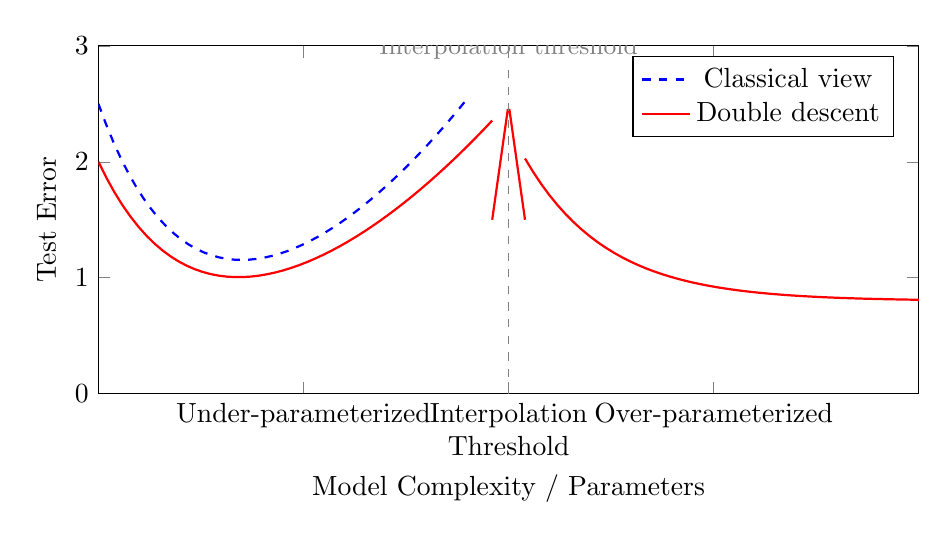
\begin{tikzpicture}
    \begin{axis}[
        xlabel={Model Complexity / Parameters},
        ylabel={Test Error},
        xmin=0, xmax=10,
        ymin=0, ymax=3,
        width=12cm,
        height=6cm,
        xtick={2.5, 5, 7.5},
        xticklabels={Under-parameterized, Interpolation\\Threshold, Over-parameterized},
        xticklabel style={align=center},
        legend pos=north east
    ]

    % Classical U-curve
    \addplot[domain=0:4.5, samples=50, thick, blue, dashed] {0.5 + 2*exp(-x) + 0.1*x^2};
    \addlegendentry{Classical view}

    % Double descent
    \addplot[domain=0:4.8, samples=50, thick, red] {0.5 + 1.5*exp(-x) + 0.08*x^2};
    \addplot[domain=4.8:5.2, samples=20, thick, red, forget plot] {2.5 - 5*abs(x-5)};
    \addplot[domain=5.2:10, samples=50, thick, red, forget plot] {0.8 + 1.5*exp(-(x-5))};
    \addlegendentry{Double descent}

    % Interpolation threshold annotation
    \draw[dashed, gray] (axis cs:5, 0) -- (axis cs:5, 2.8);
    \node[above, font=\small, gray] at (axis cs:5, 2.8) {Interpolation threshold};

    \end{axis}
\end{tikzpicture}
\caption{Double descent: Test error peaks at interpolation threshold, then decreases again in over-parameterized regime.}
\label{fig:double_descent}
\end{figure}

\subsection{Three Regimes}

\begin{enumerate}
    \item \textbf{Under-parameterized} ($p < n$): Classical regime, bias-variance trade-off applies
    \item \textbf{Interpolation threshold} ($p \approx n$): Model barely fits training data, maximum variance, worst generalization
    \item \textbf{Over-parameterized} ($p \gg n$): Many solutions fit training data, optimization finds ``good'' ones
\end{enumerate}

\subsection{Why Over-parameterization Helps}

\begin{keyinsight}[Implicit Regularization]
In the over-parameterized regime:
\begin{enumerate}
    \item Many weight configurations achieve zero training loss
    \item Gradient descent with specific initialization finds solutions with small norm
    \item Small-norm solutions tend to be smoother and generalize better
\end{enumerate}
The optimization algorithm provides implicit regularization.
\end{keyinsight}

\begin{interviewq}
\textbf{Q: Explain double descent. Why does test error decrease again in the over-parameterized regime?}

\badgeLfive{L5} \quad \badgetype{Conceptual} \quad \badgefreq{\freqhigh}

\stronganswer
Double descent describes how test error behaves as model capacity increases, revealing three distinct regimes that contradict the classical U-shaped bias-variance curve:

\begin{enumerate}
    \item \textbf{Under-parameterized} ($p < n$): Classical regime. Increasing parameters reduces bias faster than it increases variance, so test error decreases. Eventually variance dominates and test error rises---the familiar U-curve.
    \item \textbf{Interpolation threshold} ($p \approx n$): The model has just enough capacity to fit training data exactly, but is forced into a unique, fragile solution with maximum variance. This is the worst-case generalization point.
    \item \textbf{Over-parameterized} ($p \gg n$): Many weight configurations achieve zero training loss. Gradient descent with standard initialization (small random weights) converges to the minimum-norm interpolating solution, which tends to be smoother and generalizes better. This is \textit{implicit regularization}---the optimizer, not explicit regularization, selects good solutions.
\end{enumerate}

The key insight is geometric: at the interpolation threshold, the solution is unique and often high-norm (jagged). With more parameters, the solution space becomes a high-dimensional manifold, and SGD navigates to a smooth, low-norm point on that manifold.

Double descent also occurs along the \textbf{epoch axis}: test error can peak mid-training, then decrease again with further training, even after the model has memorized the data.

\redflags
\begin{itemize}
    \item Saying ``more parameters always means more overfitting'' (the classical view that double descent refutes)
    \item Not being able to explain \textit{why} over-parameterized models generalize (implicit regularization, minimum-norm solutions)
    \item Confusing interpolation threshold with overfitting (overfitting is gradual; the threshold is a specific capacity point)
\end{itemize}

\interviewtest{Whether you understand modern generalization theory beyond classical bias-variance, and can explain why scaling up models works.}

\goodgreat
\begin{itemize}
    \item \badgeLfive{L5} Describes the three regimes, identifies implicit regularization as the key mechanism.
    \item \badgeLsix{L6} Explains epoch-wise double descent, connects to the lottery ticket hypothesis (over-parameterization helps find good subnetworks), discusses practical implications for model sizing.
    \item \badgeLseven{L7} Discusses the role of data distribution structure (low-dimensional manifold), connects to benign overfitting theory, and explains how regularization (weight decay, dropout) shifts the interpolation threshold and changes the severity of the peak.
\end{itemize}

\followups{``Does double descent happen with epochs too?'' (Yes---epoch-wise double descent is observed.) ``Does regularization eliminate the peak?'' (It can reduce or shift it, but does not eliminate the phenomenon.) ``How does this relate to scaling laws?'' (Scaling laws describe the over-parameterized regime where more capacity reliably improves performance.)}
\end{interviewq}

\medskip

\begin{interviewq}
\textbf{Q: Your 10B parameter model is clearly overparameterized for your task. Should you reduce it?}

\badgeLsix{L6} \quad \badgetype{Trade-off} \quad \badgefreq{\freqhigh}

\stronganswer
The answer is almost certainly \textbf{no}---not during training. Over-parameterization is a feature, not a bug, and reducing the model prematurely can hurt performance. Here is the reasoning:

\textbf{Arguments for keeping the large model}:
\begin{enumerate}
    \item \textbf{Better optimization landscape}: Over-parameterized models have fewer bad local minima and saddle points. The loss landscape is smoother, making SGD more likely to find good solutions.
    \item \textbf{Implicit regularization}: SGD in over-parameterized models converges to minimum-norm solutions that generalize well. Reducing capacity can force the model into worse solutions.
    \item \textbf{Double descent}: Reducing from 10B toward the interpolation threshold can actually \textit{increase} test error.
    \item \textbf{Lottery ticket hypothesis}: The large model contains good subnetworks; training the full model helps find them.
    \item \textbf{Feature learning}: Larger models learn richer representations that transfer better to related tasks.
\end{enumerate}

\textbf{When to consider reducing}:
\begin{itemize}
    \item \textbf{Inference cost}: If serving cost is the bottleneck, train large, then \textit{compress}: pruning (remove 80--90\% of weights), distillation (train a smaller student from the large teacher), or quantization (INT4/INT8).
    \item \textbf{Training cost}: If you cannot afford to train a 10B model, this is a valid constraint. But the solution is a smaller model trained on more data (Chinchilla-style), not reducing parameters arbitrarily.
    \item \textbf{Severe overfitting on tiny data}: If you have $<$1K examples, a 10B model will memorize them. But the fix is usually more data or few-shot prompting, not a smaller model.
\end{itemize}

The principled approach: \textbf{train large, deploy small}. Use the over-parameterized model for training, then apply structured pruning, knowledge distillation, or quantization for deployment.

\redflags
\begin{itemize}
    \item ``Yes, reduce it to avoid overfitting'' (classical thinking that does not apply in the over-parameterized regime)
    \item Ignoring the inference cost concern (the one legitimate reason to prefer smaller models)
    \item Not knowing about post-training compression techniques
\end{itemize}

\interviewtest{Understanding of modern generalization theory, ability to distinguish training-time vs. inference-time concerns, and practical engineering judgment.}

\goodgreat
\begin{itemize}
    \item \badgeLfive{L5} Explains why over-parameterization helps (implicit regularization, better optimization), recommends train-large-deploy-small.
    \item \badgeLsix{L6} Discusses specific compression techniques with trade-offs (pruning vs. distillation vs. quantization), knows when over-parameterization can hurt (tiny data regimes).
    \item \badgeLseven{L7} Connects to the lottery ticket hypothesis and neural architecture search, discusses how the answer changes with scale (at 1T parameters, even training cost matters), and mentions that the optimal strategy depends on the ratio of training cost to lifetime inference cost.
\end{itemize}

\followups{``When does over-parameterization actually hurt?'' (When data is extremely limited and no pretraining is used; when training compute is the binding constraint.) ``How do you decide between pruning and distillation?'' (Pruning preserves the original model's architecture; distillation allows a different architecture optimized for serving. Distillation generally gives better quality at the same size.)}
\end{interviewq}

\section{Scaling Laws}
\label{sec:scaling_laws}

\subsection{Empirical Scaling Laws}

\begin{mathresult}{Kaplan et al. Scaling Laws}
Test loss follows power laws:
\begin{align}
L(N) &\propto N^{-\alpha_N} \quad \text{(parameters)} \\
L(D) &\propto D^{-\alpha_D} \quad \text{(data)} \\
L(C) &\propto C^{-\alpha_C} \quad \text{(compute)}
\end{align}
where $\alpha_N \approx 0.076$, $\alpha_D \approx 0.095$, $\alpha_C \approx 0.050$ for language models.
\end{mathresult}

These exponents are small, and converting them to intuition is an interview move in itself: with $\alpha_C \approx 0.05$, a $10\times$ increase in compute reduces loss by only a factor of $10^{0.05} \approx 1.12$ (about 11\%), and $2\times$ compute buys roughly 3--4\%. Loss improvements from scale are reliable but expensive.

\subsection{Chinchilla Scaling}

\begin{mathresult}{Chinchilla Optimal Scaling}
For a fixed compute budget $C$:
\begin{equation}
N_{opt} \propto C^{0.5}, \quad D_{opt} \propto C^{0.5}
\end{equation}
Optimal ratio: $D \approx 20N$ (tokens $\approx$ 20 × parameters)
\end{mathresult}

\textbf{Implication}: GPT-3 (175B params, 300B tokens) was undertrained. Chinchilla (70B params, 1.4T tokens) outperforms both GPT-3 and its compute-matched sibling Gopher (280B) at the same training budget as Gopher.

\subsection{The Joint Parametric Form and How Scaling Laws Are Fit}
\label{sec:scaling_fitting}

The single-variable power laws above are slices of a joint loss surface. The form Chinchilla actually fit---and the one to write down when asked to design a scaling study---is:

\begin{mathresult}{Chinchilla Joint Parametric Form}
\begin{equation}
L(N, D) = E + \frac{A}{N^{\alpha}} + \frac{B}{D^{\beta}}
\end{equation}
with fitted values (Hoffmann et al., 2022): $E \approx 1.69$, $A \approx 406$, $B \approx 411$, $\alpha \approx 0.34$, $\beta \approx 0.28$.
\end{mathresult}

Each term has a meaning: $E$ is the irreducible entropy of the data---the floor an infinite model trained on infinite data would reach; $A/N^{\alpha}$ is the penalty for finite capacity; $B/D^{\beta}$ is the penalty for finite data. Minimizing $L(N,D)$ subject to $C = 6ND$ (a one-line Lagrange calculation) gives $N_{\text{opt}} \propto C^{\beta/(\alpha+\beta)}$ and $D_{\text{opt}} \propto C^{\alpha/(\alpha+\beta)}$; with $\alpha \approx \beta$, both exponents are $\approx 0.5$---which is exactly where ``scale $N$ and $D$ together'' and the 20:1 ratio come from.

\textbf{The three fitting approaches.} Chinchilla ran all three; their mutual agreement is the actual evidence for the 20:1 rule:
\begin{enumerate}
    \item \textbf{Fixed-$N$ sweeps}: Train a grid of model sizes, each over a range of token counts. For each compute budget, read off which $(N, D)$ pair achieved the minimum loss, then fit $N_{\text{opt}}(C)$ through those minima.
    \item \textbf{IsoFLOP profiles}: Fix several total budgets $C$ and vary $N$ (with $D = C/6N$). Loss vs.\ $N$ at fixed $C$ traces a parabola on a log axis; its minimum is $N_{\text{opt}}(C)$. This is the cleanest visualization and the standard picture in scaling papers.
    \item \textbf{Parametric fit}: Fit $L(N,D) = E + A/N^{\alpha} + B/D^{\beta}$ directly to all runs (in practice: a Huber loss on log-space residuals, minimized from a grid of initializations to avoid bad local optima), then optimize the fitted surface analytically.
\end{enumerate}

\begin{warningbox}
Every fit point must come from a run whose learning-rate schedule was \textit{completed} at that token count. Reading intermediate losses off one long run silently inflates them (the LR has not yet decayed), and this---together with omitting embedding parameters in the parameter count at small scale---is a large part of why Kaplan et al.\ (2020) concluded $N_{\text{opt}} \propto C^{0.73}$ (scale model size much faster than data) while Chinchilla's corrected fits gave $C^{0.5}$. The two papers disagreed about experimental method, not about nature.
\end{warningbox}

\subsection{Implications for Practice}

\begin{table}[H]
\centering
\caption{Scaling law implications}
\begin{tabularx}{\textwidth}{lX}
\toprule
\textbf{Finding} & \textbf{Practical Implication} \\
\midrule
Power law in parameters & 10× params → predictable improvement \\
Power law in data & More data always helps (diminishing returns) \\
Compute-optimal scaling & Balance model size and training data \\
Transfer across tasks & Scaling laws similar across domains \\
\bottomrule
\end{tabularx}
\end{table}

\begin{interviewq}
\textbf{Q: Your team has a fixed compute budget. How do you decide model size vs. training data?}

\badgeLsix{L6} \quad \badgetype{Trade-off} \quad \badgefreq{\freqhigh}

\stronganswer
This is the core question that Chinchilla scaling laws address. For a fixed compute budget $C \propto 6ND$ (where $N$ = parameters, $D$ = tokens), the compute-optimal allocation scales both model size and data as $C^{0.5}$:
\[N_{\text{opt}} \propto C^{0.5}, \quad D_{\text{opt}} \propto C^{0.5}\]

The practical rule: \textbf{tokens $\approx$ 20$\times$ parameters}. This means most early LLMs were \textit{undertrained}:
\begin{itemize}
    \item GPT-3: 175B params, 300B tokens (ratio 1.7:1)---vastly undertrained
    \item Chinchilla: 70B params, 1.4T tokens (ratio 20:1)---matches GPT-3 (175B) quality with $\sim$2.5$\times$ cheaper inference; the famous 4$\times$ figure is vs.\ its compute-matched sibling Gopher (280B)
\end{itemize}

\textbf{However}, Chinchilla-optimal is not always the right target. The decision depends on whether you optimize for training cost or inference cost:
\begin{itemize}
    \item \textbf{Training-cost-optimal} (Chinchilla): Use the 20:1 ratio. Best if you retrain frequently.
    \item \textbf{Inference-cost-optimal} (LLaMA/Mistral approach): Train a \textit{smaller} model on \textit{more} data than Chinchilla prescribes. You ``waste'' training compute but get a cheaper-to-serve model. LLaMA-3 8B was trained on 15T tokens (ratio 1875:1).
\end{itemize}

If you cannot get more data: do not scale the model beyond what your data supports. Instead, invest in data quality (filtering, deduplication, curriculum) or use synthetic data augmentation.

\redflags
\begin{itemize}
    \item Citing only the Chinchilla ratio without considering inference cost trade-offs
    \item Saying ``just use the biggest model possible'' without considering data availability
    \item Not knowing the approximate 20:1 ratio or the $C \approx 6ND$ relationship
\end{itemize}

\interviewtest{Knowledge of scaling laws, ability to make cost-aware engineering decisions, and understanding of training vs. inference trade-offs.}

\goodgreat
\begin{itemize}
    \item \badgeLfive{L5} Knows Chinchilla scaling, cites the 20:1 ratio.
    \item \badgeLsix{L6} Distinguishes training-optimal from inference-optimal, gives concrete examples (LLaMA, Chinchilla), discusses data quality.
    \item \badgeLseven{L7} Discusses how scaling laws break down (data quality ceilings, diminishing returns at frontier scale, domain-specific data scarcity), connects to the ``over-training'' regime and when it is economically rational (amortized inference cost dominates training cost for widely-deployed models).
\end{itemize}

\followups{``What if you have unlimited data but limited inference budget?'' (Train a smaller model longer---over-train relative to Chinchilla.) ``How do you estimate compute cost?'' ($C \approx 6ND$ for a forward + backward pass; multiply by number of epochs.) ``Do scaling laws transfer across domains?'' (Broadly yes, but exponents differ; vision and code have different optimal ratios.)}
\end{interviewq}

\medskip

\begin{interviewq}
\textbf{Q: Estimate the compute-optimal model size for a training budget of $10^{22}$ FLOPs using Chinchilla scaling laws.}

\badgeLsix{L6} \quad \badgetype{Estimation} \quad \badgefreq{\freqhigh}

\stronganswer
Using the Chinchilla compute law $C \approx 6ND$ (where $C$ = FLOPs, $N$ = parameters, $D$ = tokens), and the optimal ratio $D \approx 20N$:

\textbf{Step 1}: Substitute $D = 20N$ into $C = 6ND$:
\[C = 6N \cdot 20N = 120N^2\]

\textbf{Step 2}: Solve for $N$:
\[N = \sqrt{\frac{C}{120}} = \sqrt{\frac{10^{22}}{120}} = \sqrt{8.33 \times 10^{19}} \approx 9.1 \times 10^9 \approx \textbf{9B parameters}\]

\textbf{Step 3}: Compute optimal tokens:
\[D = 20N \approx 20 \times 9\text{B} = \textbf{180B tokens}\]

\textbf{Sanity check}: $C = 6 \times 9 \times 10^9 \times 180 \times 10^9 = 9.7 \times 10^{21} \approx 10^{22}$ FLOPs. This checks out.

\textbf{Context}: $10^{22}$ FLOPs is roughly 18{,}000 A100 GPU-hours at 50\% MFU ($312 \times 10^{12} \times 0.5 \times 3600 = 5.6 \times 10^{17}$ FLOPs per GPU-hour, so $10^{22} / 5.6 \times 10^{17} \approx 18{,}000$ GPU-hours---e.g., 1,000 A100s for 18 hours). At typical cloud prices ($\sim$\$1--4 per A100-hour), that is roughly \$20--70k. This is a modest training run by industry standards.

\textbf{Caveat}: The Chinchilla ratio optimizes for minimal training compute at a given loss. If inference cost matters more (model will be deployed at scale), you should train a smaller model on more data (LLaMA-style: 7B on 1T+ tokens).

\redflags
\begin{itemize}
    \item Not knowing the $C \approx 6ND$ approximation
    \item Getting the arithmetic wrong (practice powers-of-10 calculations)
    \item Treating Chinchilla ratios as a universal law rather than an empirical guideline (exponents vary by domain and data quality)
\end{itemize}

\interviewtest{Can you do back-of-envelope estimation using scaling laws? Do you understand the practical implications?}

\goodgreat
\begin{itemize}
    \item \badgeLfive{L5} Knows the $D \approx 20N$ rule and arrives at the right order of magnitude.
    \item \badgeLsix{L6} Derives from $C = 6ND$, performs the sanity check, contextualizes in GPU-hours, and mentions the inference-cost caveat.
    \item \badgeLseven{L7} Discusses how the optimal ratio shifts with data quality (high-quality data has a lower optimal ratio), explains the $6ND$ derivation (2 FLOPs per multiply-add $\times$ 3 passes: forward + backward for weights and activations), and discusses how recent work (Llama 3, DeepSeek) operates far beyond Chinchilla-optimal.
\end{itemize}

\followups{``Where does $C = 6ND$ come from?'' (Each parameter participates in $\sim$2 FLOPs per token in the forward pass; backward pass costs $\sim$2$\times$ forward; total $\approx 6$ FLOPs per parameter per token.) ``How would your answer change for a code model vs. a language model?'' (Code data is higher quality per token; you may want a larger model trained on less data, or equivalently, the optimal ratio may be closer to 10:1.)}
\end{interviewq}

\medskip

\begin{interviewq}
\textbf{Q: You get 1\% of the target training budget to run scaling experiments that must predict the final run's loss. Design the study.}

\badgeLseven{L7} \quad \badgetype{Architecture Design} \quad \badgefreq{\freqmed}

\stronganswer
Frame the budget first: if the target run costs $C$, the study gets $0.01C$. That is enough for $\sim$20 runs spanning two-plus orders of magnitude of compute below the target---provided the largest experiment stays around $10^{-3}C$ and a reserve is kept for reruns.

\textbf{Design:}
\begin{enumerate}
    \item \textbf{Freeze everything that must match the target}: tokenizer, data mixture (same sampling weights, same dedup pipeline), architecture family, context length. If the mixture or preprocessing shifts between the small runs and the target, the fit is invalid before it starts.
    \item \textbf{IsoFLOP grid}: Pick $\sim$4 compute budgets logarithmically spaced (e.g., $10^{-5}C$ to $3 \times 10^{-3}C$); at each, train $\sim$5 model sizes spanning roughly an order of magnitude around the expected optimum, with $D = C_i/6N$. Total $\approx 0.7\%$ of $C$, leaving reserve.
    \item \textbf{Scale hyperparameters, do not copy them}: every run gets its own \textit{completed} LR decay to its final token count (never intermediate checkpoints of a longer run); peak LR is re-tuned per scale or transferred in a principled way ($\mu$P); batch size stays below the critical batch size at every scale so the compute accounting is honest.
    \item \textbf{Fit}: $L(N,D) = E + A/N^{\alpha} + B/D^{\beta}$ with a Huber loss on log-residuals from a grid of initializations; cross-check against the IsoFLOP-minima fit (Section~\ref{sec:scaling_fitting})---the two should agree.
    \item \textbf{Validate before believing}: hold out the largest compute tier, fit on the rest, and check the prediction error on the held-out tier; bootstrap the fit for a confidence interval. Report predicted loss as a band, not a point---you are extrapolating $\sim$2 orders of magnitude.
    \item \textbf{Deliverable}: $N_{\text{opt}}$, $D_{\text{opt}}$, predicted loss $\pm$ CI, plus the explicit caveat that the fit predicts \textit{loss} only---downstream benchmark accuracy does not extrapolate (see the emergence discussion).
\end{enumerate}

\textbf{Failure modes} (the standard follow-up is ``your extrapolation missed by 2$\times$---why?''):
\begin{itemize}
    \item \textbf{LR schedule not scaled}: fit points taken from intermediate checkpoints of one cosine run, or one peak LR reused across all scales (the optimum shifts with scale unless you use $\mu$P).
    \item \textbf{Mixture shift across scales}: small runs on a convenience subset with different composition, or multi-epoch at small scale while the target is single-epoch.
    \item \textbf{Fitting range too narrow}: an exponent fitted over 1--1.5 orders of magnitude and extrapolated over 2+ amplifies small exponent errors exponentially.
    \item Batch size above the critical batch size at some scales (wasted FLOPs corrupt the compute axis); evaluation noise at the smallest scales dominating the fit.
\end{itemize}

\redflags
\begin{itemize}
    \item ``Train one small model and scale its loss by the textbook exponent'' (no fit, no uncertainty, wrong exponents for your data)
    \item Using intermediate losses of a single long run as fit points (the Kaplan-vs-Chinchilla lesson)
    \item Promising benchmark scores from a loss extrapolation
\end{itemize}

\interviewtest{Can you design an experiment under a hard budget constraint, and do you know where scaling-law fits break in practice? This distinguishes having read Chinchilla from having reproduced it.}

\goodgreat
\begin{itemize}
    \item \badgeLfive{L5} Knows the idea: several small runs, fit a power law, extrapolate.
    \item \badgeLsix{L6} Designs an IsoFLOP grid, insists on completed LR schedules per point, fits the joint parametric form, and cross-checks two fitting approaches.
    \item \badgeLseven{L7} Validates on a held-out compute tier with bootstrap uncertainty, uses $\mu$P for hyperparameter transfer, knows the Kaplan-vs-Chinchilla methodology story, budgets a rerun reserve, and states explicitly what the study cannot predict.
\end{itemize}

\followups{``Your extrapolation came in 2$\times$ off---list causes in priority order.'' (LR schedule not scaled, mixture shift across scales, fitting range too narrow, batch size off the critical-batch curve.) ``How does $\mu$P change this study?'' (Hyperparameters tuned at small width transfer to large width, removing the per-scale LR sweep.) ``The target run will repeat data---does the fit still hold?'' (Not directly; see the data-constrained scaling discussion below.)}
\end{interviewq}

\medskip

\begin{interviewq}
\textbf{Q: Neural scaling laws: what scales and what does not? When do they break?}

\badgeLseven{L7} \quad \badgetype{Conceptual} \quad \badgefreq{\freqmed}

\stronganswer
\textbf{What scales predictably} (smooth power laws):
\begin{itemize}
    \item \textbf{Cross-entropy loss} as a function of parameters ($N$), data ($D$), and compute ($C$): $L(N) \propto N^{-\alpha_N}$, $L(D) \propto D^{-\alpha_D}$, $L(C) \propto C^{-\alpha_C}$
    \item \textbf{Upstream metrics}: Perplexity, bits-per-byte---they track loss closely
    \item \textbf{Consistent across modalities}: Language, vision, code, multimodal---power law exponents differ but the functional form holds
\end{itemize}

\textbf{What does NOT scale predictably}:
\begin{itemize}
    \item \textbf{Downstream task accuracy}: Performance on specific benchmarks (e.g., MMLU, GSM8K) does not follow clean power laws. Small improvements in loss can yield large accuracy gains (or none) depending on the task's difficulty threshold.
    \item \textbf{Safety and alignment}: Larger models are not automatically safer; some failure modes (sycophancy, persuasion capability) get worse with scale.
    \item \textbf{Reasoning chains}: Multi-step reasoning quality scales less predictably than pattern matching or knowledge recall.
    \item \textbf{Calibration}: Does not degrade with scale the way folklore suggests---larger \textit{base} models are typically \textit{better} calibrated; the well-documented overconfidence appears after RLHF post-training, which degrades calibration (GPT-4 system card).
\end{itemize}

\textbf{When scaling laws break}:
\begin{enumerate}
    \item \textbf{Data quality ceiling}: With web-scraped data, returns diminish after $\sim$10T tokens because of repetition and noise. High-quality curated or synthetic data has different (better) scaling exponents.
    \item \textbf{Architecture matters}: Scaling laws assume fixed architecture. Architectural innovations (MoE, better attention) shift the curve---the same loss at lower compute.
    \item \textbf{Domain-specific limits}: Some domains have inherent complexity ceilings (e.g., formal verification) where more data does not help without algorithmic improvements.
    \item \textbf{Post-training}: RLHF, instruction tuning, and chain-of-thought can improve downstream performance without changing the base model's loss---these are ``scaling'' improvements that scaling laws do not capture.
    \item \textbf{Compute-efficiency frontiers}: Hardware changes (better GPUs, communication, compilers) shift what is practically achievable at a given dollar cost, even if FLOP-based laws hold.
\end{enumerate}

\redflags
\begin{itemize}
    \item Treating scaling laws as deterministic laws of nature rather than empirical trends
    \item Conflating loss scaling with downstream task scaling
    \item Ignoring the role of data quality and architecture
\end{itemize}

\interviewtest{Nuanced understanding of when first-principles reasoning about scale applies and when it breaks down.}

\goodgreat
\begin{itemize}
    \item \badgeLfive{L5} Knows the power law form and Chinchilla scaling.
    \item \badgeLsix{L6} Distinguishes loss scaling from task scaling, discusses data quality limitations.
    \item \badgeLseven{L7} Discusses architecture-dependent scaling (MoE has different exponents), post-training contributions that bypass scaling laws, and how to use scaling laws for practical compute budgeting (fit a power law on small runs to predict large-run performance, with appropriate uncertainty bounds).
\end{itemize}

\followups{``How would you use scaling laws to plan a training run?'' (Train 3--5 small models at different scales, fit the power law, extrapolate to target compute. Add safety margin for distribution shift between small and large scale.) ``Do scaling laws hold for fine-tuning?'' (Approximately yes for loss, but with different exponents and higher sensitivity to data quality.)}
\end{interviewq}

\subsection{Data-Constrained Scaling}
\label{sec:data_constrained}

Chinchilla assumes unlimited fresh data: every one of the $D$ tokens is unique. The 2026 reality is different---frontier runs already consume most of the usable web---so the binding question became: \textit{what happens when you must repeat data?} Muennighoff et al.\ (2023) answered it quantitatively by training hundreds of models at varying unique-data budgets and epoch counts:

\begin{itemize}
    \item \textbf{Up to $\sim$4 epochs, repetition is nearly free}: loss after 4 passes over $D$ unique tokens is almost indistinguishable from one pass over $4D$ fresh tokens.
    \item \textbf{Returns decay rapidly after that}: they fit an effective-data form in which the marginal value of a repeated token decays exponentially with epoch count.
    \item \textbf{Past $\sim$16 epochs, additional repetition is essentially worthless}: extra compute spent on more passes buys no loss reduction---the model has extracted what the corpus contains.
    \item Under a data constraint, the compute-optimal allocation shifts: relative to naive Chinchilla on the unique-token count, train \textit{smaller models for more epochs} rather than scaling parameters into data the model will only memorize.
\end{itemize}

\textbf{The ceiling.} Estimates of usable, deduplicated, quality-filtered web text land around 10--20T tokens. Frontier pretraining runs already train on 15--40T tokens, so the 4-epoch grace period stretches the wall to perhaps 50--80T effective tokens---while compute budgets keep growing on a much faster schedule than the web does.

\textbf{What labs do at the wall:}
\begin{enumerate}
    \item \textbf{Mine non-web pools}: code and multilingual corpora add tens of trillions of tokens and improve reasoning and transfer beyond their own domains.
    \item \textbf{Synthetic data with verification}: model-generated math and code filtered by execution, checkers, or verifiers; rephrased and textbook-style corpora. Verifiability is the load-bearing word---unverified synthetic data risks degenerate self-training loops, which is why math and code lead this wave.
    \item \textbf{Curation over collection}: aggressive dedup, filtering, and quality weighting shift the effective scaling exponents---the same loss from fewer, better tokens.
    \item \textbf{Spend compute on a different axis}: epochs to the $\sim$4-epoch point, then inference-time compute (next subsection).
\end{enumerate}

\begin{keyinsight}[Epochs Are Nearly Free, Until They Are Worthless]
Repeating the corpus up to $\sim$4 epochs costs almost nothing relative to fresh data; by $\sim$16 epochs, further repetition contributes essentially zero. ``We are running out of web data'' therefore really means ``we are running out of cheap epochs'': the wall sits $\sim$4$\times$ further out than single-epoch accounting suggests---and then it is genuinely a wall, which is why frontier labs pivot to code, multilingual, and verified synthetic data rather than more passes.
\end{keyinsight}

\subsection{The Third Axis: Test-Time Compute}
\label{sec:third_axis}

Until 2024, ``scaling'' meant two train-time axes: parameters $N$ and data $D$. Reasoning models (OpenAI o1 in 2024, DeepSeek-R1 in 2025) opened a third: \textbf{FLOPs spent per query at inference}. RL on verifiable rewards trains models to emit long chains of thought before answering, and accuracy on reasoning benchmarks then scales roughly log-linearly with the compute spent thinking---a lever that exists \textit{after} training is finished. In the Chinchilla frame: train-time compute buys a better per-token distribution; test-time compute spends extra forward passes to extract more reliability from a fixed model. The two are partially fungible, which breaks the old assumption that capability is fixed at training time.

Sequential scaling spends the budget on one longer chain of thought---deliberation, self-checking, backtracking---and pays in \textit{latency}, since thinking tokens are generated serially. Parallel scaling spends it on $N$ independent samples plus a selection rule (best-of-$N$ against a verifier or reward model, self-consistency majority voting) and pays in \textit{throughput} while keeping wall-clock latency near a single generation.

\textbf{Compute-optimal test-time scaling} (Snell et al., 2024): at a fixed inference-FLOP budget, the optimal split between model size and per-query search is \textit{difficulty-dependent}. On easy and medium problems, a smaller model plus many samples and a selector beats a much larger model sampled once, because the small model's coverage (pass@$N$) is already high and selection converts coverage into accuracy. On the hardest problems, coverage is the binding constraint---pass@$N$ stays near zero no matter how large $N$---and no selection mechanism can help; capability must come from parameters and training. The selector is also a ceiling of its own: against an imperfect verifier, large $N$ increasingly harvests false positives---Goodhart's law at inference time.

\textbf{When it substitutes for parameters---and when it cannot.} Test-time compute substitutes for model size when the task is verifiable (or a good selector exists), base-model coverage is nonzero, and the latency budget tolerates thinking. It does \textit{not} substitute for knowledge: a small model cannot think its way to facts it never stored, so recall-heavy workloads still scale with parameters (or get retrieval instead). Economically, total cost $=$ training $+$ inference $\times$ queries now contains a per-query knob set at serving time: ``what size model should we train'' becomes entangled with a routing and thinking-budget policy---cheap fast paths for easy queries, deliberation for hard ones.

The machinery behind this axis---GRPO and RL on verifiable rewards, the R1 training recipe, budget forcing, best-of-$N$ and verifier-based selection, and the serving implications of decode-heavy reasoning workloads---is covered in Section~\ref{sec:reasoning_ttc} of Chapter~\ref{chap:reinforcement_learning}; the prompting-side view (chain-of-thought and self-consistency as user-level techniques) is in the NLP volume (see [NLP 7], Volume II). The reason this subsection exists is that no 2026 scaling answer may stop at Chinchilla: ``how would you spend $10\times$ more compute'' now has three legitimate answers---bigger $N$, more $D$, or more inference---and a strong candidate weighs all three.

\section{The Lottery Ticket Hypothesis}
\label{sec:lottery_ticket}

\textbf{Lottery Ticket Hypothesis.} Dense, randomly-initialized networks contain sparse subnetworks (``winning tickets'') that, when trained in isolation from the same initialization, can match the full network's performance.

\subsection{Key Findings}

\begin{enumerate}
    \item \textbf{Existence}: Winning tickets exist (found via iterative pruning)
    \item \textbf{Initialization matters}: Must use original initialization, not random re-init
    \item \textbf{Sparsity}: Can prune 90-95\% of weights while maintaining accuracy
    \item \textbf{Transferability}: Tickets transfer across datasets (somewhat)
\end{enumerate}

\subsection{Implications}

\begin{itemize}
    \item Over-parameterization helps find good subnetworks
    \item Pruning after training can recover efficient models
    \item Motivates neural architecture search and efficient architectures
\end{itemize}

\section{Grokking}
\label{sec:grokking}

\textbf{Grokking.} The phenomenon where a model achieves perfect training accuracy long before achieving good generalization, with generalization suddenly improving much later in training.

\begin{figure}[H]
\centering
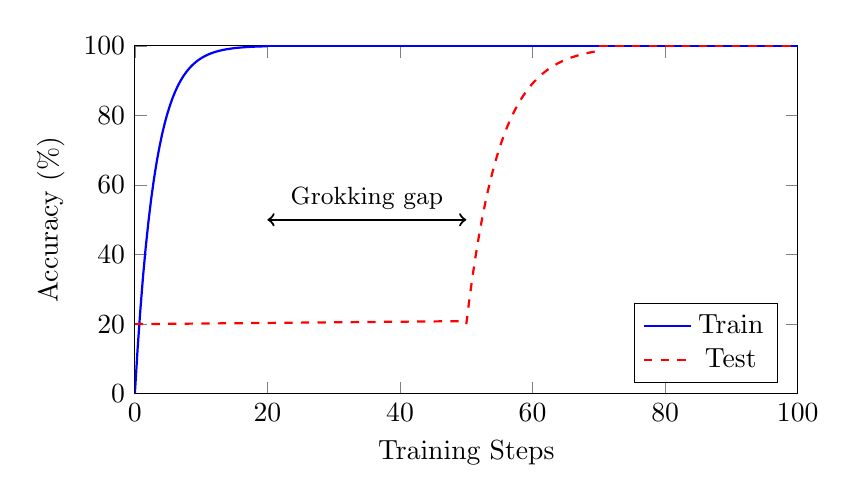
\begin{tikzpicture}
    \begin{axis}[
        xlabel={Training Steps},
        ylabel={Accuracy (\%)},
        xmin=0, xmax=100,
        ymin=0, ymax=100,
        legend pos=south east,
        width=10cm,
        height=6cm
    ]

    % Training accuracy
    \addplot[domain=0:20, samples=50, thick, blue] {100*(1 - exp(-x/3))};
    \addplot[domain=20:100, samples=50, thick, blue, forget plot] {100};
    \addlegendentry{Train}

    % Test accuracy (grokking)
    \addplot[domain=0:50, samples=50, thick, red, dashed] {20 + 10*sin(x/10)};
    \addplot[domain=50:70, samples=50, thick, red, dashed, forget plot] {20 + 80*(1 - exp(-(x-50)/5))};
    \addplot[domain=70:100, samples=50, thick, red, dashed, forget plot] {100};
    \addlegendentry{Test}

    % Annotations
    \draw[<->, thick] (20, 50) -- (50, 50) node[midway, above, font=\small] {Grokking gap};

    \end{axis}
\end{tikzpicture}
\caption{Grokking: Training accuracy saturates early, test accuracy improves much later.}
\end{figure}

\subsection{When Grokking Occurs}

\begin{itemize}
    \item Small datasets with algorithmic structure (modular arithmetic)
    \item Heavy regularization (weight decay critical)
    \item Long training (much longer than needed for memorization)
\end{itemize}

\subsection{Proposed Explanations}

\begin{enumerate}
    \item \textbf{Representation learning}: Network first memorizes, then learns generalizable features
    \item \textbf{Circuit formation}: Generalizing circuits form slowly alongside memorizing circuits
    \item \textbf{Regularization dynamics}: Weight decay gradually removes memorization
\end{enumerate}

\begin{interviewq}
\textbf{Q: What is grokking and what does it tell us about generalization?}

\badgeLsix{L6} \quad \badgetype{Conceptual} \quad \badgefreq{\freqmed}

\stronganswer
\textbf{Grokking} (Power et al., 2022) is the phenomenon where a neural network achieves perfect training accuracy long before achieving good generalization, with a dramatic, sudden improvement in test accuracy far later in training---often $10\times$--$100\times$ more training steps after memorization.

\textbf{When it occurs}:
\begin{itemize}
    \item Small datasets with underlying algorithmic structure (modular arithmetic, group operations, permutations)
    \item Weight decay is critical---grokking rarely occurs without it
    \item Long training well past the point of memorization
\end{itemize}

\textbf{What it tells us about generalization}:
\begin{enumerate}
    \item \textbf{Memorization and generalization are separate mechanisms}: The network first memorizes training data using high-complexity features, then gradually discovers simpler, generalizable representations. These two solutions coexist during training.
    \item \textbf{Regularization drives the transition}: Weight decay slowly penalizes the high-norm memorization circuit, eventually making the low-norm generalization circuit dominant. Without weight decay, the model stays in the memorization solution.
    \item \textbf{Representation learning takes time}: The generalizing solution requires discovering the underlying algebraic structure, which takes many more gradient steps than brute-force memorization.
    \item \textbf{Phase transitions in learning}: Generalization can improve discontinuously---relevant to understanding emergent abilities in LLMs.
\end{enumerate}

\textbf{Mechanistic interpretability connection}: Studies using circuit analysis show that grokking involves the formation of ``clean'' circuits (e.g., Fourier features for modular addition) that gradually replace ``messy'' memorization circuits. This is one of the clearest examples of feature learning dynamics we can study.

\redflags
\begin{itemize}
    \item Describing grokking as just ``training longer helps''---the key is the \textit{sudden} transition, not gradual improvement
    \item Not mentioning the role of weight decay
    \item Treating it as a curiosity rather than connecting it to broader generalization theory
\end{itemize}

\interviewtest{Understanding of generalization dynamics beyond static bias-variance analysis, and awareness of recent ML theory developments.}

\goodgreat
\begin{itemize}
    \item \badgeLfive{L5} Describes the phenomenon accurately, knows weight decay is required.
    \item \badgeLsix{L6} Explains the two-phase mechanism (memorization then generalization), connects to regularization dynamics and circuit formation.
    \item \badgeLseven{L7} Discusses the mechanistic interpretability findings (Fourier features for modular arithmetic), connects to phase transitions in learning, and discusses whether grokking-like phenomena occur at LLM scale (evidence suggests yes---some capabilities emerge late in training, especially with continued pretraining).
\end{itemize}

\followups{``Does grokking happen in large models?'' (Not typically observed at scale with standard training, but analogous delayed generalization phenomena do occur---e.g., capabilities emerging late in training.) ``Could you engineer grokking to be faster?'' (Yes---increasing weight decay, using data augmentation on the algorithmic task, or using specific learning rate schedules can accelerate the transition.)}
\end{interviewq}

\section{Emergent Abilities}
\label{sec:emergent}

\textbf{Emergent Abilities.} Capabilities that appear suddenly at certain model scales, being absent in smaller models and present in larger ones, with sharp transitions rather than gradual improvement.

\subsection{Examples}

\begin{table}[H]
\centering
\caption{Commonly cited emergence thresholds---as reported in 2022, with their current status}
\begin{tabularx}{\textwidth}{lXX}
\toprule
\textbf{Ability} & \textbf{2022-era threshold} & \textbf{Status by 2026} \\
\midrule
In-context learning & $\sim$10B params (GPT-3-era recipes) & Routine in sub-1B models trained on modern data mixtures \\
Instruction following & $\sim$10B params & Sub-1B instruct-tuned models follow instructions competently \\
Chain-of-thought reasoning & $\sim$100B params & Distilled 1.5B reasoning models produce coherent multi-step chains \\
\bottomrule
\end{tabularx}
\end{table}

Read the middle column as an \textbf{artifact of that era's training recipes}, not a property of scale itself. The 2022 thresholds were measured on models trained on lightly filtered web text with no instruction data, no reasoning traces, and no distillation. Once a capability has been discovered at scale, better data (instruction mixes, curated chain-of-thought) and distillation reliably move it into models 10--100$\times$ smaller---exactly what the metric-artifact reading of emergence predicts. Quote the historical numbers as data points about 2022 recipes, never as laws. The debate itself has also moved: the 2026 version asks whether RL post-training \textit{creates} new capabilities or \textit{elicits} ones already latent in the base model (the pass@$k$ vs.\ pass@1 argument)---see Chapter~\ref{chap:reinforcement_learning}.

\subsection{Debate on Emergence}

Recent work questions whether emergence is ``real'' or an artifact of:
\begin{itemize}
    \item \textbf{Discrete evaluation metrics}: Accuracy shows sharp transitions that look like emergence
    \item \textbf{Smooth underlying improvement}: Continuous metrics (log-likelihood) show gradual, predictable gains across all scales
    \item \textbf{Task-difficulty thresholds}: Compositional tasks appear ``emergent'' because success requires all sub-steps to exceed a threshold simultaneously
\end{itemize}

\begin{interviewq}
\textbf{Q: Are emergent abilities in LLMs real, or an artifact of evaluation?}

\badgeLsix{L6} \quad \badgetype{Conceptual} \quad \badgefreq{\freqmed}

\stronganswer
This is genuinely debated in the research community, and a strong answer presents both sides.

\textbf{The emergence claim} (Wei et al., 2022): Certain capabilities---chain-of-thought reasoning, in-context learning, multi-step arithmetic---appear suddenly at specific model scales, with near-zero performance below the threshold and sharp improvement above it.

\textbf{The artifact argument} (Schaeffer et al., 2023):
\begin{itemize}
    \item ``Emergence'' only appears with \textit{discrete, nonlinear} metrics (exact match accuracy) that show sharp transitions
    \item With \textit{continuous} metrics (log-likelihood, token-level accuracy, Brier score), improvement is smooth and predictable across all scales
    \item The ``emergence'' is in the metric, not the model---it is a measurement artifact of thresholding continuous improvement
    \item Changing the metric (e.g., from exact match to partial credit) eliminates the appearance of emergence
\end{itemize}

\textbf{The nuanced reality}:
\begin{itemize}
    \item Even if individual sub-skills improve smoothly, their \textit{composition} can produce emergent behavior. Solving a 5-step math problem requires all 5 steps to be correct; if each step's accuracy improves gradually from 80\% to 99\%, the chain's success rate jumps from $0.8^5 = 33\%$ to $0.99^5 = 95\%$
    \item Qualitatively, the capability to perform multi-step reasoning does appear at a specific scale in practice, even if continuous metrics improve smoothly
    \item Emergence may be ``real'' at the task level while being ``artificial'' at the metric level
\end{itemize}

\textbf{Interview-safe conclusion}: Emergence is partly real (compositional capabilities do appear at scale) and partly metric artifact (smooth improvement looks sharp under discrete metrics). The practical implication: you cannot reliably predict when a capability will appear, so evaluate at multiple scales and use continuous metrics when possible.

\redflags
\begin{itemize}
    \item Taking an extreme position (``emergence is completely fake'' or ``emergence is magical'')
    \item Not knowing the Schaeffer et al. critique
    \item Conflating ``emergence'' with ``scaling laws'' (scaling laws predict smooth improvement; emergence is about discontinuities)
\end{itemize}

\interviewtest{Critical thinking about ML claims and ability to evaluate conflicting research evidence.}

\goodgreat
\begin{itemize}
    \item \badgeLfive{L5} Describes the phenomenon and knows it is debated.
    \item \badgeLsix{L6} Presents both sides with specific citations, explains the metric artifact argument.
    \item \badgeLseven{L7} Discusses the compositional-skills explanation, connects to phase transitions in statistical physics, and explains practical implications for model development (you need to evaluate at many scales, and small models are unreliable proxies for large-model capabilities on compositional tasks).
\end{itemize}

\followups{``How would you test if a capability is truly emergent?'' (Use continuous metrics, test at many intermediate scales, decompose into sub-skills and check if each improves smoothly.) ``Does this affect how you plan model training?'' (Yes---you cannot rely on small-scale experiments to predict large-model capabilities for compositional tasks.)}
\end{interviewq}

\section{Implicit Regularization of SGD}
\label{sec:implicit_reg}

\subsection{Flat vs. Sharp Minima}

\begin{figure}[H]
\centering
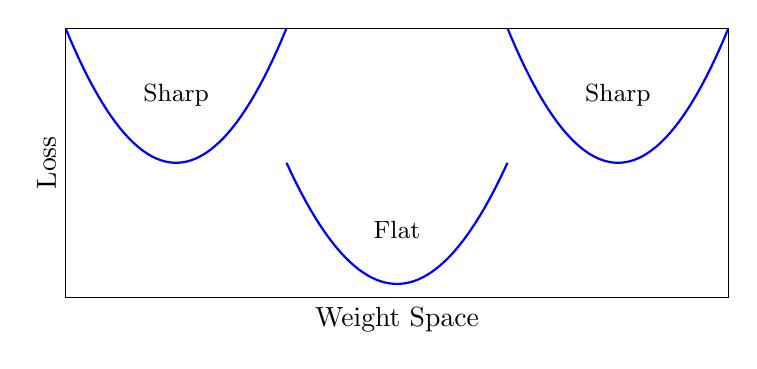
\begin{tikzpicture}
    \begin{axis}[
        xlabel={Weight Space},
        ylabel={Loss},
        xmin=-3, xmax=3,
        ymin=0, ymax=2,
        width=10cm,
        height=5cm,
        xtick=\empty,
        ytick=\empty
    ]

    % Sharp minimum
    \addplot[domain=-3:-1, samples=50, thick, blue] {1 + (x+2)^2};
    \addplot[domain=-1:1, samples=50, thick, blue] {0.1 + 0.9*(x)^2};
    \addplot[domain=1:3, samples=50, thick, blue] {1 + (x-2)^2};

    % Labels
    \node[font=\small] at (-2, 1.5) {Sharp};
    \node[font=\small] at (0, 0.5) {Flat};
    \node[font=\small] at (2, 1.5) {Sharp};

    % Arrows indicating generalization
    \draw[->, thick, green!70!black] (0, -0.3) -- (0, 0) node[below=0.3cm, font=\small] {Better generalization};

    \end{axis}
\end{tikzpicture}
\caption{Flat minima generalize better than sharp minima.}
\end{figure}

\subsection{Why SGD Finds Flat Minima}

\begin{enumerate}
    \item \textbf{Noise from mini-batches}: Gradient noise helps escape sharp minima
    \item \textbf{Learning rate}: Larger LR → more noise → flatter minima
    \item \textbf{Batch size}: Smaller batches → more noise → flatter minima
\end{enumerate}

\begin{keyinsight}
The ratio $\frac{\eta}{B}$ (learning rate / batch size) controls the ``temperature'' of SGD. Higher temperature explores more and finds flatter minima.
\end{keyinsight}

\subsection{Connection to Generalization}

Flat minima generalize better because:
\begin{itemize}
    \item Small perturbations (distribution shift) don't increase loss much
    \item Robust to noise in test data
    \item Often correspond to simpler functions
\end{itemize}

\begin{warningbox}
Classical statistical learning theory (VC dimension, Rademacher complexity) predicts over-parameterized models should overfit catastrophically. Deep learning violates these predictions routinely. In interviews, don't apply classical generalization bounds to deep networks---instead, discuss implicit regularization, double descent, and the role of optimization in finding good solutions.
\end{warningbox}

\begin{interviewq}
\textbf{Q: Training loss is still decreasing but validation loss plateaued. You have $10\times$ more unlabeled data available. What do you do?}

\badgeLsix{L6} \quad \badgetype{Trade-off} \quad \badgefreq{\freqmed}

\stronganswer
Diagnose carefully before naming the disease: a \textit{plateaued} validation loss while training loss keeps falling means a \textbf{growing generalization gap}---suggestive of overfitting but ambiguous, since a plateau can also mean you have hit a capacity or data ceiling. The definitive overfitting signal is validation loss \textit{rising}. Either way, labeled data is the binding constraint here, and $10\times$ more unlabeled data opens several strategies, ordered by likely impact:

\textbf{Strategy 1: Continued (domain-adaptive) pretraining (most impactful)}
\begin{itemize}
    \item Start from an existing foundation model and continue pretraining on the unlabeled corpus with a self-supervised objective (next-token prediction, masked language modeling, or contrastive learning depending on domain)
    \item Then fine-tune on the labeled data. Pretraining \textit{from scratch} on the unlabeled corpus alone is rarely the right call today---reserve it for domains with no usable foundation model
    \item This leverages the unlabeled data to learn general representations, dramatically reducing the effective sample complexity of the downstream task
    \item This is the foundation of modern transfer learning and is almost always the right first move
\end{itemize}

\textbf{Strategy 2: Semi-supervised learning}
\begin{itemize}
    \item Use the current model to pseudo-label the unlabeled data (self-training)
    \item Filter pseudo-labels by confidence threshold
    \item Retrain on the combined labeled + pseudo-labeled data
    \item Risk: confirmation bias (model reinforces its own errors). Mitigate with iterative refinement and diversity in the pseudo-labeled set.
\end{itemize}

\textbf{Strategy 3: Data augmentation}
\begin{itemize}
    \item Use the unlabeled data to train augmentation models (e.g., back-translation for NLP, style transfer for vision)
    \item Apply augmentation to expand the effective labeled dataset
\end{itemize}

\textbf{Strategy 4: Regularization (if above is not feasible)}
\begin{itemize}
    \item Increase dropout, weight decay, or add label smoothing
    \item Apply early stopping at the validation plateau
    \item Reduce model size (last resort---see discussion on over-parameterization)
\end{itemize}

\textbf{What NOT to do}: Simply continue training unchanged---validation performance has stalled, and the fix lies in the data, not more steps. Be careful with ``make it bigger'' too: with the labeled set fixed and small, a larger model mostly widens the train-val gap. Note this is a heuristic, not a law---per the double descent section, bigger-plus-regularized can generalize better, especially once the unlabeled data is put to work.

\redflags
\begin{itemize}
    \item ``Just train longer'' (validation performance has stalled---more steps attack the wrong constraint)
    \item ``Make the model bigger'' as the first move (capacity is not the bottleneck; without leveraging the unlabeled data, scaling the model attacks the wrong constraint)
    \item Ignoring the $10\times$ unlabeled data---the interviewer gave this information for a reason
    \item Jumping to ``reduce the model'' without first trying to leverage the unlabeled data
\end{itemize}

\interviewtest{Practical ML engineering judgment---can you diagnose the problem, prioritize solutions, and leverage available resources (unlabeled data)?}

\goodgreat
\begin{itemize}
    \item \badgeLfive{L5} Identifies overfitting, suggests pretraining or semi-supervised learning.
    \item \badgeLsix{L6} Presents strategies in priority order, discusses trade-offs (pretraining cost vs. semi-supervised noise), mentions specific techniques (pseudo-labeling with confidence filtering).
    \item \badgeLseven{L7} Discusses the interplay between model scale and data regime (when is pretraining cost-effective vs. semi-supervised), considers domain-specific factors (medical imaging where unlabeled data is plentiful but labels are expensive), and mentions active learning as an alternative (label the most informative unlabeled examples if a labeling budget exists).
\end{itemize}

\followups{``What if the unlabeled data is from a different domain?'' (Domain adaptation techniques: gradual fine-tuning, domain-adversarial training, or using it only for representation learning with a domain-specific head.) ``How would you decide between pretraining and pseudo-labeling?'' (Pretraining is better when the domain gap between labeled and unlabeled is small and you have compute. Pseudo-labeling is cheaper and works when the model is already reasonably accurate.)}
\end{interviewq}

%==============================================================================
\section{Why Large Models Generalize}
\label{sec:why_large_generalize}
%==============================================================================

First, get the regime right---interviewers probe exactly this. LLM \textit{pretraining} is roughly single-epoch online learning: GPT-3 saw $\sim$300B tokens with 175B parameters (more tokens than parameters, not the reverse), each token roughly once; training loss never reaches zero, and the train-test gap is small because every batch is effectively fresh data. Classic $p \gg n$ overfitting reasoning therefore applies mainly to \textit{fine-tuning} and vision-style multi-epoch training, where models genuinely can interpolate the training set. It is in that over-parameterized regime that classical statistical learning theory (VC dimension, Rademacher complexity) predicts catastrophic overfitting, yet models generalize well. Several complementary explanations resolve this paradox:

\begin{enumerate}
    \item \textbf{Implicit regularization of gradient descent}: For linear models trained from small initialization, (full-batch) gradient descent provably converges to minimum-norm interpolating solutions; deep networks show a similar implicit bias empirically. These solutions are smoother and generalize better. The optimization algorithm itself acts as a regularizer---the inductive bias is in the optimizer, not the architecture alone. (This norm-minimization mechanism is distinct from the mini-batch-noise mechanism in the next item.)
    \item \textbf{Flat minima}: SGD noise (from mini-batches) biases optimization toward flat regions of the loss landscape. Flat minima are robust to perturbations (distribution shift between train and test), explaining good generalization. The ``temperature'' of SGD ($\propto \eta/B$) controls this effect.
    \item \textbf{Compression during training (contested)}: Information-bottleneck analyses report that after an initial fitting phase, networks enter a compression phase where representations become more compact and task-relevant. Treat this as a hypothesis, not settled fact---replications (Saxe et al., 2018) found the compression phase depends on the activation function and the mutual-information estimator.
    \item \textbf{Data structure}: Real-world data lies on low-dimensional manifolds despite living in high-dimensional spaces. The effective complexity of the learning problem is much lower than the ambient dimensionality suggests. A 175B parameter model is not ``overparameterized'' for the true complexity of natural language.
    \item \textbf{Benign overfitting}: In high-dimensional settings, a model can perfectly interpolate training data while remaining smooth between data points. The ``extra'' parameters enable the model to fit noise in directions orthogonal to the signal subspace, without corrupting predictions.
\end{enumerate}

\begin{interviewq}
\textbf{Q: Why do large language models generalize despite having more parameters than training examples?}

\badgeLseven{L7} \quad \badgetype{First Principles} \quad \badgefreq{\freqmed}

\stronganswer
Start by interrogating the premise---this is where strong candidates separate. LLM \textit{pretraining} is roughly single-epoch: GPT-3 trained on $\sim$300B tokens with 175B parameters, so it did not literally have more parameters than training examples; its loss never reached zero, and the train-test gap is small because online SGD on effectively fresh data barely overfits. The genuine puzzle lives in the over-parameterized regime ($p \gg n$)---fine-tuning, vision-style multi-epoch training, small-data settings---where classical statistical learning theory (VC dimension, Rademacher complexity) predicts catastrophic overfitting yet models generalize. Several complementary explanations exist:

\textbf{1. Implicit regularization of SGD}: Gradient descent does not find arbitrary interpolating solutions---from small initialization it converges to \textit{minimum-norm} solutions (for linear models, provably; for neural nets, empirically). These solutions are smoother and lower-complexity than the worst-case solutions that classical theory considers. The optimization algorithm itself is a regularizer.

\textbf{2. Data lies on low-dimensional manifolds}: Natural language, despite living in a vocabulary-sized discrete space, has far lower intrinsic dimensionality. The effective number of ``free parameters'' the model needs to learn is much smaller than $N$. A 70B parameter model is not overparameterized for the \textit{intrinsic} complexity of natural language.

\textbf{3. Flat minima and PAC-Bayes}: SGD's noise biases it toward flat regions of the loss landscape. Flat minima correspond to solutions where small weight perturbations do not change predictions---this is precisely the condition for generalization under distribution shift. PAC-Bayes bounds, which account for the ``sharpness'' of the minimum, give much tighter generalization guarantees than VC-dimension bounds.

\textbf{4. Compression and information bottleneck (contested)}: One line of work argues that representations undergo a compression phase where task-irrelevant information is discarded, so effective model complexity (description length, Fisher information) is far below the raw parameter count. Cite it with the caveat that the compression phase failed to replicate robustly (Saxe et al., 2018).

\textbf{5. Benign overfitting}: In high-dimensional settings, a model can fit training noise in directions orthogonal to the signal subspace without affecting generalization. The ``extra'' parameters absorb noise without corrupting the learned function along relevant directions.

\textbf{6. Structural priors in the architecture}: Transformers have strong inductive biases (locality via attention patterns, compositionality via residual stream, smoothness via the embedding space) that restrict the effective hypothesis class even when the raw parameter count is enormous.

No single explanation is complete; these are complementary lenses on the same phenomenon.

\redflags
\begin{itemize}
    \item ``They don't generalize---they just memorize'' (empirically false; LLMs generate novel, coherent text)
    \item Citing VC dimension as the reason to expect overfitting without acknowledging its limitations
    \item Giving only one explanation (this is a multi-faceted phenomenon)
\end{itemize}

\interviewtest{Depth of theoretical understanding, ability to reason about open problems, and awareness of the gap between classical theory and modern practice.}

\goodgreat
\begin{itemize}
    \item \badgeLfive{L5} Mentions implicit regularization and that classical theory does not apply directly.
    \item \badgeLsix{L6} Discusses 3+ complementary explanations (implicit regularization, data manifolds, flat minima), connects to double descent.
    \item \badgeLseven{L7} Discusses PAC-Bayes as a theoretically-grounded alternative to VC theory, explains benign overfitting, and acknowledges what we still do not understand (e.g., why specific architectures generalize better than others with the same parameter count, why pretraining on seemingly unrelated data helps downstream tasks).
\end{itemize}

\followups{``What is PAC-Bayes and why does it give tighter bounds?'' (PAC-Bayes bounds depend on the distance between the learned model and a prior over models, not the raw hypothesis class size. Flat minima have small PAC-Bayes bounds.) ``Is memorization always bad?'' (No---LLMs memorize factual knowledge, which is essential for utility. The question is whether they memorize noise, which they largely do not.)}
\end{interviewq}
